\chapter{Overall Description}
\section{Product Perspective}
\subsection{Scenarios}

\subsubsection{Creating a tournament}
Chip, a professor of Algorithm and Data Structures at Mouseton Institute of Technology prepared to teach the chapter on strings, launching the "Strings Operations" coding tournament on CKB.
To expand participation, he allowed his colleague Dale to create challenges for his software engineering class.
STUs across classes would compete in string manipulation tasks, ranging from basic concatenation to advanced text analysis, fostering collaboration and learning.
To make the tournament more interesting, Chip decided to award badges to the best-performing STUs, so he added badges for the STUs who participate in most tournaments, one for the STUs who win most battles, and one for the STUs who write most lines of code.
All STUs already subscribed to CKB were notified of the new tournament, and they could join it from the tournament page till a defined deadline.

\subsubsection{Creating a battle}
In order to familiarize STUs with the CKB platform and its features, Chip created an easy battle for his STUs to practice, called "Wordcheck".
The task essentially required STUs to implement the game Wordle in the C language.
He decided that the battle would last for two weeks, allowing STUs to work in teams of 1 up to 3 people. STUs would be able to join the battle until the deadline's last day.\\
In addition, he wanted to give extra points for code cleanup.
Therefore, he had to review the code of each team at the end of the battle and assign extra points to the teams that wrote clean code.
Chip set all this information in the battle creation form and then created the battle.

\subsubsection{Joining a battle}
Huey and Dewey, two STUs of Chip's class, are notified of an incoming battle and decide to join it.
Since the more the merrier, they decide to invite their friend Louie to join them in the battle.
Louie receives the invitation mail and decides to join the battle in their team.
After the registration deadline, they are notified that the battle is about to start.
They get the link to the GitHub repository of the battle to fork it and then set up an automated workflow to link their GitHub account to the CKB platform. \\
After the automated workflow is set up, they are ready to start working on the battle.

\subsubsection{Improving the score and obtaining a badge}
Donald is another warrior of the "Wordcheck" battle and he is working on the battle alone.
After the first commit, he logs in to the CKB to check his score.
He sees that he is in the 3rd position and that he is 10 points behind the leading team, composed of Huey, Dewey, and Louie.
Fortunately, the battle is still in progress and the CKB platform allows him to improve his score by pushing new commits to the GitHub repository, so he decides to work on the battle for a couple of days and then push his updated work to the GitHub repository.
After checking his score again, he is now in the 1st position and moreover, he obtained a badge for being the first to reach 100 points in the battle.
From now on, both STUs and professors can see this badge when they visit Donald's profile.

\subsubsection{Closing a battle}
When the deadline for the battle created by Chip is reached, all participants are notified that the battle is closed and that they can not push new commits to their GitHub repository.
Chip can now evaluate the code of each team and assign extra points for the clarity of the comments and the code, as he decided when he created the battle.
After the evaluation, the final rank of the battle is available to all participants, and the STUs are notified that they can now see the final rank of the battle.

\subsubsection{Closing a tournament}
Chip decides to close the "Strings Operations" tournament when all the battles end.
To do so, he logs into the CKB platform and he closes the tournament.
All participants are notified that the tournament is closed, in the end, the CKB platform makes the final rank of the tournament available to all participants.

\subsubsection{Accessing the scores of the players}
Huey wishes to enroll in the class Advanced Algorithms and Data Structures held by Professor Pippo, so he applies for the class.
Pippo, who wants to make sure that Huey is a good STU, comes to know that Huey is a very active user of the CKB platform and he decides to check his profile.
He sees that Huey has a very high score in the "Strings Operations" tournament and that he has a badge for being the most active user of the platform, he also notes that Huey is involved in more than one tournament simultaneously.
Thanks to the CKB platform, Pippo now has a complete overview of Huey's skills and he can decide whether to accept his application or not.

\subsubsection{Creating Game badges}
Scrooge, a Software Engineering professor at Duckburg University, believes that, in addition to the existing badges in the CKB platform, it would be nice to introduce badges for STUs who achieve a perfect score in a battle and a tournament.
Since the CKB platform allows EDUs to create new badges, he creates the two badges and from now on, all EDUs will have the option to include these badges in their tournaments and battles.

\subsection{Class Diagram}
Figure \ref{fig:class-diagram} represents a simplified view of the UML class diagram of the system.
This is not a comprehensive view of all the classes needed, but rather a view to capture the general composition and the different relations between them.
In particular, the most important details are:
\begin{itemize}
    \item There are only two possible types of users: STU and EDU type.
    \item EDUs can create tournaments and battles, moreover, they can grant permission to create battles to other colleagues inside their own tournament.
    \item STUs can subscribe to tournament and battles, invite other STUs to form teams, and achieves badges, using both the CKB platform and GitHub.
          The most important detail is subscribing to a battle: STUs can join a battle by creating their own team (a team is composed respecting imposed boundaries) or by joining an existing team.
          In particular, the team class exists iff a battle exists, i.e. a team exists only in the battle scope.
    \item Tournament and Battle classes use the MailAPI to notify STUs about events.
\end{itemize}

\begin{figure}[H]
    \centering
    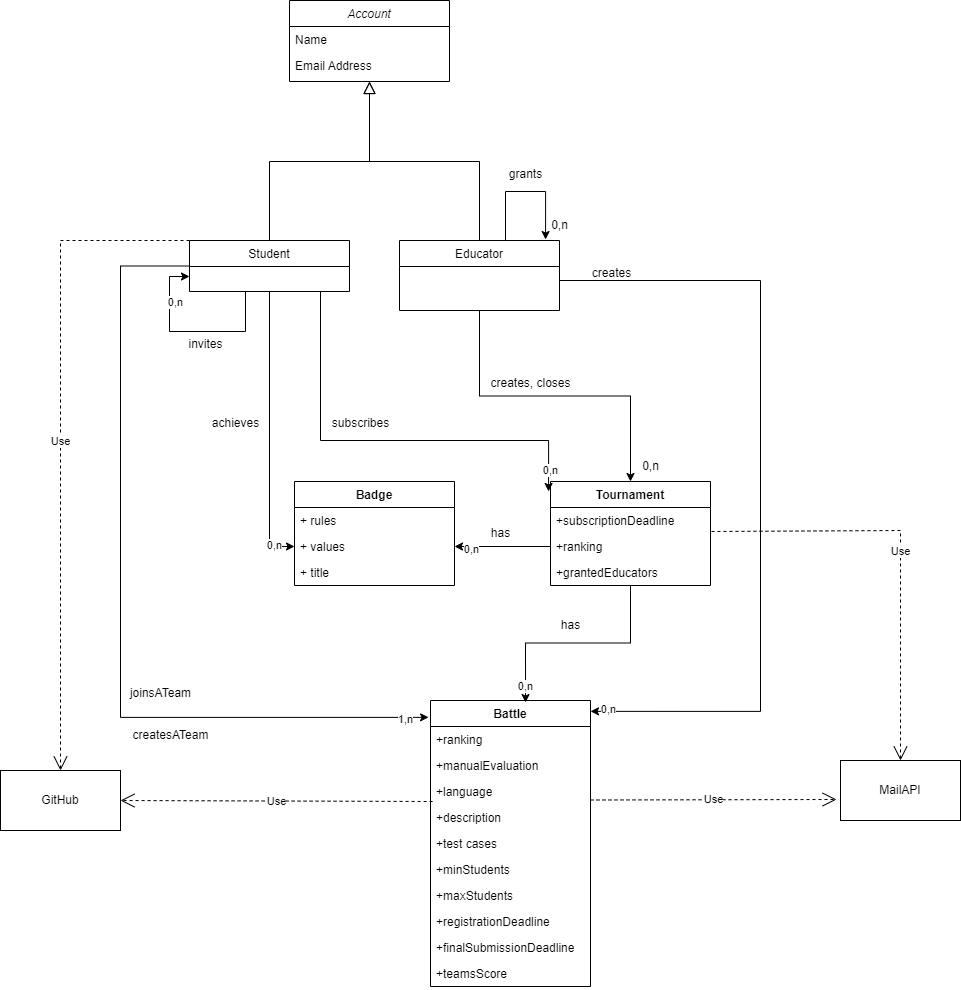
\includegraphics[width=0.8\textwidth]{images/state_diagrams/ClassDiagram.png}
    \caption{Class Diagram}
    \label{fig:class-diagram}
\end{figure}

\subsection{State Diagrams}
The following state diagrams describe the life cycle of the main entities of the system.
Moreover, they specify the sequence of states that an object goes through during its lifetime in response to stimuli from the environment.
We want to focus on the events that cause a transition from one state to another and the actions that result from a state change.

\subsubsection*{Tournament}
After an EDU creates a tournament, it is both in the \textit{registration open} and \textit{tournament open} states.\\
In the \textit{registration open} state, STUs can join the tournament, while in the \textit{tournament open} state, EDUs with the right permissions can create battles within the tournament, and that leads the tournament to the \textit{battling} state.\\
When the deadline for registration is reached, the tournament moves to the \textit{registration closed} state and no more STUs can join it.\\
When the deadline for the registrations is reached, no more STUs can join the tournament and it moves permanently to the \textit{registration closed} state.\\
During the \textit{battling} state EDUs can start multiple parallel battles or can finally close the tournament, iff all battles are ended.\\
The diagram is shown in figure \ref{fig:tournament-state-diagram}.

\subsubsection*{Battle}
The battle evolves linearly, starting from the \textit{registration open} immediately followed by the \textit{registration closed} state.\\
After the registration deadline is reached, the GitHub repository of the battle is created and thus the battle moves to the \textit{coding} state, allowing the STUs to fork the repository and start working on the battle.\\
When the deadline for the battle is reached, the EDUs can start evaluating the code of the STUs, if previously enabled (\textit{consolidation} state). \\
After the evaluation is completed, the battle can be closed and the final rank is available to all participants.\\
The diagram is shown in figure \ref{fig:battle-state-diagram}.

\subsubsection*{Score evaluation}
The score evaluation of a battle is a process that is triggered by the end of a battle and it is composed of multiple steps.\\
First, three aspects can be automatically evaluated: functional aspects (the higher the better, +), timeliness (the lower the better, -), and quality level of the sources, extracted through static analysis tools (+). \\
Finally, if the EDU enabled the manual evaluation, it can assign extra points. \\
The diagram is shown in figure \ref{fig:score-evaluation-state-diagram}.

\begin{figure}[H]
    \centering
    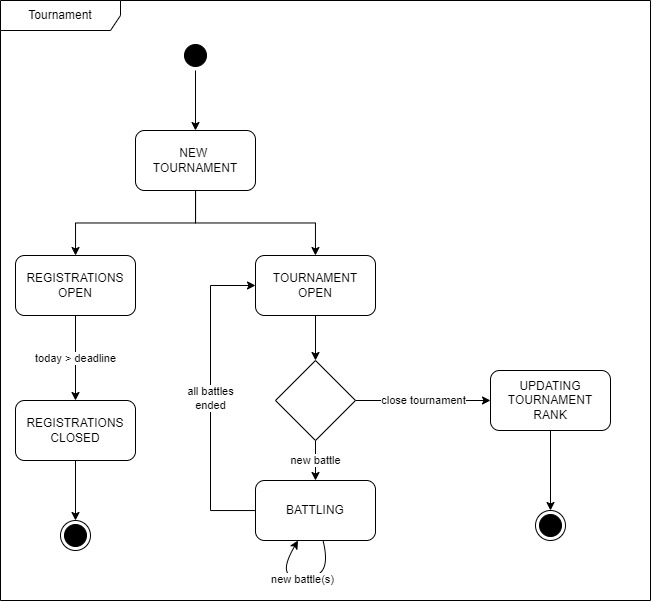
\includegraphics[width=.8\textwidth]{images/state_diagrams/tournament.jpg}
    \caption{Tournament state diagram}
    \label{fig:tournament-state-diagram}
\end{figure}
\begin{figure}[H]
    \centering
    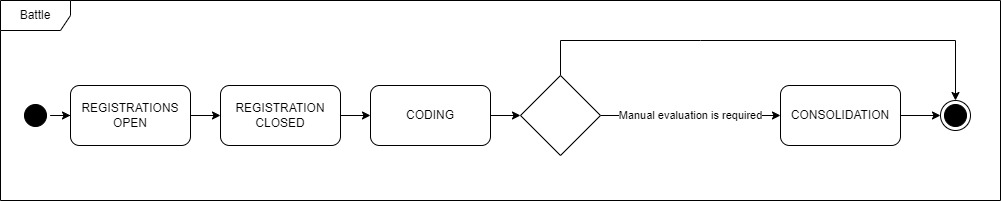
\includegraphics[width=1\textwidth]{images/state_diagrams/battle.jpg}
    \caption{Battle state diagram}
    \label{fig:battle-state-diagram}
\end{figure}
\begin{figure}[H]
    \centering
    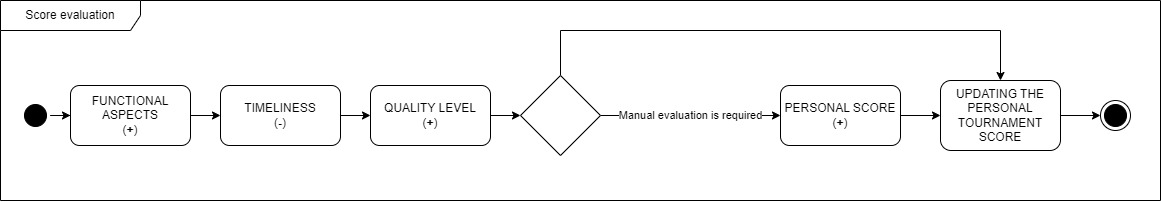
\includegraphics[width=1\textwidth]{images/state_diagrams/score_evaluation.jpg}
    \caption{Score evaluation state diagram}
    \label{fig:score-evaluation-state-diagram}
\end{figure}

\section{Product Functions}
\subsection{Register function}
A user approaching CKB for the first time can register on the platform.
The information necessary for the system to keep track of users is personal data such as Name, Surname, Email, School they belong to, and what role they hold in the school environment (STU / EDU).
This last information is very important as it guarantees two types of accounts with different rights and duties.

By expressing that it is an EDU, all rights related to the creation of tournaments, battles, and badges are guaranteed.
By choosing a STU account, it can actively participate in tournaments and battles and earn badges.

\subsection{Create tournament function}
To create a tournament, an EDU registered in the CKB platform must define all the required information.
The tournament needs:
\begin{itemize}
    \item a name.
    \item a time window aimed at welcoming STU registrations.
    \item a list of badges that STUs can obtain during the whole tournament duration.
\end{itemize}

\subsection{Creating battles function}
In the context of an active tournament, any authorized EDU can decide to create a battle that will be managed by itself.
New battles require:
\begin{itemize}
    \item the programming language to solve the problem.
    \item the test cases that must be passed by each team's code, at the end of the battle.
    \item the build automation scripts correctly set.
    \item the specification of the problem to be solved including at least one example to achieve a test-first approach.
    \item the deadline for the battle registration period.
    \item the deadline for the conclusion of the battle.
    \item the type of evaluation method, in particular, set manual evaluation in addition to the automatic one performed by the platform.
    \item constraints for the maximum and minimum number of players required for each team.
\end{itemize}

\subsection{Join tournament and battles function}
STUs registered on the platform receive notification every time a new tournament is created and can decide whether to participate.
Likewise, in the context of a tournament in which they applied, they are informed of new upcoming battles.
Registration for a battle can be done in various ways as long as it is before the end of the registration window.

\subsection{Gamification function}
EDUs, at any time, can create a new badge by defining a title and a rule.
Once a badge is created, it will be available on the CKB platform for every EDU who wishes to use it in a new tournament.
When creating a tournament, the EDU specifies the list of included badges from those available.
At the end of the tournament in which they are enrolled, STUs receive the badges for which the specified rule has been satisfied.
The same badge can be assigned to more than one STU.

\section{User characteristics}
Users of the system fall into one of the following categories: STU or EDU.

\subsection*{STU}
STUs participate actively in Code Kata tournaments and battles to enhance their software development skills.
During a battle, STUs develop solutions following the "test-first" approach and use GitHub to manage their code.
The CKB platform automatically evaluates STU progress based on the number of tests passed, timeliness, and quality of code, providing scores updated in real-time.
STUs aim to achieve high scores and accumulate gamification badges defined by EDUs.
In addition to participating in battles, STUs can view their tournaments' rank and receive notifications on final results.
The STU's primary goal is to improve programming skills, obtain competitive scores, and earn badges through active participation in the collaborative context of the CKB platform.

\subsection*{EDU}
EDUs take a central role in directing STUs toward improving software development skills through programming competitions.
Their duties include creating tournaments and battles, finalizing challenge details, and managing STU registrations.
EDUs assign specific tasks to STUs, and then they manually evaluate STUs' solutions, contributing to the automatic evaluation of projects performed by the CKB platform of functional, temporal, and code quality aspects.
Furthermore, they can create gamification badges, and rewards based on rules established, to motivate STUs.
The main objective is to improve STUs' skills, ensuring fair and efficient assessment and encouraging active involvement.
The EDU plays a key role in educational innovation, exploring new possibilities through the definition of personalized rules and badges that stimulate growth and collaboration.
In summary, the EDU acts as a promoter of an engaging and competitive training challenge on CKB.

\section{Assumptions, Dependencies and Constraints}

\subsection{Domain Assumptions}
\begin{table}[H]
    \centering
    \renewcommand{\arraystretch}{0.5}
    \begin{tabular}{l l p{10.5cm}}
        \hline
                     &        &                                                                                                                                                                                                                                               \\
        \textbf{ID}  & \vline & \textbf{Description}                                                                                                                                                                                                                          \\
                     &        &                                                                                                                                                                                                                                               \\\hline & & \\
        \textbf{DA1} & \vline & STUs code with the programming language set for the battle they are taking part.                                                                                                                                                              \\
                     &        &                                                                                                                                                                                                                                               \\\hline & & \\
        \textbf{DA2} & \vline & EDUs upload the Code Kata with the correct description and software project, including test cases, and build automation scripts related to it.                                                                                                \\
                     &        &                                                                                                                                                                                                                                               \\\hline & & \\
        \textbf{DA3} & \vline & STUs fork the GitHub repository of the Code Kata and set up an automated workflow through GitHub Actions that informs the CKB platform (through proper API calls) as soon as STUs push a new commit into the main branch of their repository. \\
                     &        &                                                                                                                                                                                                                                               \\\hline & & \\
        \textbf{DA4} & \vline & EDUs manual evaluation ranges from 0 to 100\footnote{The full evaluation will be given by the average of all the four aspects evaluated by the CKB platform, the three automatic and the manual one}.                                         \\
                     &        &                                                                                                                                                                                                                                               \\\hline & & \\
        \textbf{DA5} & \vline & The data inserted, by users, at registration  time, are truthful.                                                                                                                                                                             \\
                     &        &                                                                                                                                                                                                                                               \\\hline & & \\
        \textbf{DA6} & \vline & GitHub and the tool for static analysis always work properly and they are reliable.                                                                                                                                                           \\
                     &        &                                                                                                                                                                                                                                               \\\hline & & \\
        \textbf{DA7} & \vline & A team is composed of at least the minimum number of people up to the maximum number defined by EDUs, if no minimum is defined it will be 1 by default.                                                                                       \\
                     &        &                                                                                                                                                                                                                                               \\\hline & & \\
        \textbf{DA8} & \vline & All users subscribed to the CKB platform have a GitHub account.                                                                                                                                                                               \\
                     &        &                                                                                                                                                                                                                                               \\
        \hline
    \end{tabular}
    \caption{Assumption}
\end{table}

\subsection{Dependencies}
\begin{table}[H]
    \centering
    \renewcommand{\arraystretch}{0.5}
    \begin{tabular}{l l p{10.5cm}}
        \hline
                      &        &                                                                                  \\
        \textbf{ID}   & \vline & \textbf{Description}                                                             \\
                      &        &                                                                                  \\\hline & & \\
        \textbf{Dep1} & \vline & The system requires an internet connection to interact with CKB and other users. \\
                      &        &                                                                                  \\\hline & & \\
        \textbf{Dep2} & \vline & The system integrates an external API to compile the code written by STUs.       \\
                      &        &                                                                                  \\\hline & & \\
        \textbf{Dep3} & \vline & The system integrates a GitHub API to create a repository for each battle        \\
                      &        &                                                                                  \\
        \hline
    \end{tabular}
    \caption{Dependencies}
\end{table}

\subsection{Constraints}
\begin{itemize}
    \item The software must follow local laws and rules, especially when it comes to handling user data, such as letting users access their data when they want.
    \item The software should only collect personal data it really needs, like just the user's name, email address, and the school it belongs to and few more.
    \item To keep users' important info safe, like passwords and personal data, it must be stored in SHA256 encoding in the database.
    \item When choosing external APIs, especially those that are crucial for it to work properly, we should pick the ones that are the most dependable and always available.
\end{itemize}